\section{Описание существующих решений}

В данном разделе будет проведён анализ существующих операционных систем для устройств интернета вещей. Рассматриваемые операционные системы будут относиться к одному из двух типов: ОС реального времени и ОС разделения времени.

\subsection{Операционные системы реального времени}

\subsubsection{Azure RTOS}

Microsoft Azure RTOS ThreadX \cite{Azure_RTOS_overview} --- это операционная система реального времени (Real-Time Operating System, RTOS) для интернета вещей и пограничных устройств, работающих на микроконтроллерах (Micro Controller Unit, MCU). Azure RTOS разработана для поддержки устройств с жесткими ограничениями по ресурсам (как правило, работающих от аккумуляторов и имеющих менее 64 КБ флэш-памяти).

Azure RTOS обеспечивает сертифицированную по Common Criteria среду безопасности EAL4+, включая полную безопасность на уровне IP через IPsec и безопасность на уровне сокетов через TLS и DTLS. Криптобиблиотека прошла сертификацию FIPS 140-2. Также реализованы аппаратные криптографические возможности, защита памяти с помощью ThreadX MODULES и поддержка функций безопасности TrustZone ARM ARMv8-M.

Одной из отличительных особенностей данной ОС является архитектура ядра, организованного по структуре пикоядра (picokernel) \cite{Azure_RTOS_picokernel}. При таком подходе службы ОС размещаются на одном уровне, что устраняет ненужные временные затраты при вызове функций.

Azure RTOS ThreadX разработана для глубоко встраиваемых приложений. Название ThreadX происходит от потоков, которые используются в качестве исполняемых элементов, а <<X>> обозначает переключение потоков. ThreadX поддерживает среды с многоядерными процессорами посредством асимметричной многопроцессорной обработки или симметричной многопроцессорной обработки. ThreadX распространяется с использованием маркетинговой модели, в которой исходный код бесплатен, а лицензии предоставляются бесплатно.

Azure RTOS используется в специализированном оборудовании, таком, как устройства беспроводной связи, принтеры, модемы, устройства хранения данных, медицинские устройства, интеллектуальные датчики.



\subsubsection{Azure Sphere}

Microsoft Azure Sphere \cite{Azure_Sphere_main} --- это специализированная операционная система для микроконтроллеров на базе Linux, созданная Microsoft для работы на чипе, сертифицированном для Azure Sphere, и для подключения к службе безопасности Azure Sphere. Операционная система Azure Sphere предоставляет платформу для разработки приложений для интернета вещей , включая как приложения высокого уровня, так и приложения, поддерживающие работу в реальном времени. Это первая операционная система с ядром Linux \cite{linux} , которую Microsoft публично выпустила, и вторая Unix-подобная операционная система, разработанная компанией для публичного пользования.

Служба безопасности Azure Sphere \cite{Azure_Sphere_terminology} \cite{Azure_Sphere_overview}, представляет собой облачную службу, которая обеспечивает обслуживание, обновление и контроль чипов, сертифицированных Azure Sphere. Служба безопасности Azure Sphere устанавливает безопасное соединение между устройствами и интернетом и/или облачными службами и обеспечивает безопасную загрузку. Основная цель контакта между устройством Azure Sphere и службой безопасности Azure Sphere --- проверка подлинности удостоверения устройства, обеспечение целостности и доверия к системному программному обеспечению, а также подтверждение того, что на устройстве работает доверенная кодовая база. Служба также предоставляет безопасный канал, используемый корпорацией Майкрософт для автоматической загрузки и установки обновлений ОС Azure Sphere и обновлений клиентских приложений на развернутые устройства.

\begin{figure}[h]
	\centering
	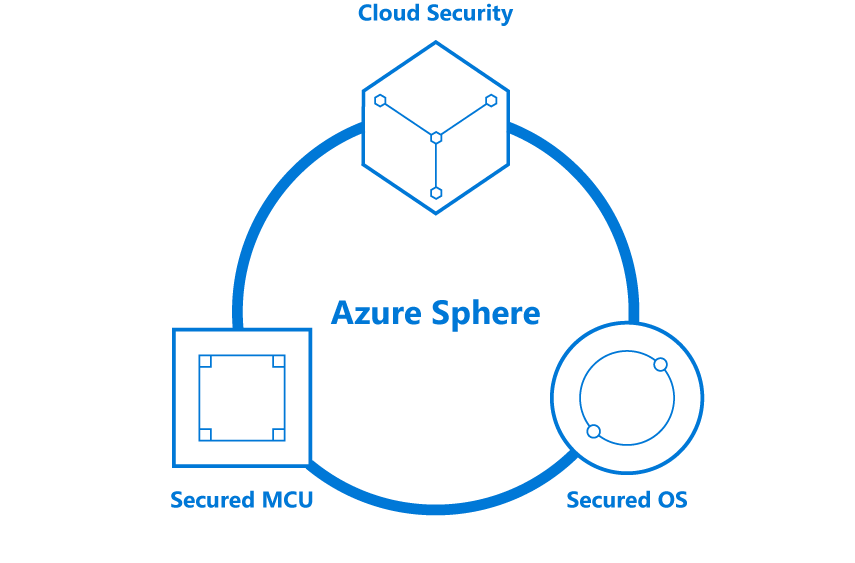
\includegraphics[width=0.85\textwidth]{img/azure-sphere.png}
	\caption{Компоненты системы на базе Azure Sphere}
	\label{fig:azure}
\end{figure} 

Согласно рисунку \ref{fig:azure} \cite{Azure_Sphere_parts}, система, основанная на Azure Sphere, состоит из трех компонентов, главный из которых --- микроконтроллер (MCU), поддерживающий семь важнейших аппаратных функций, которые, по мнению Microsoft, являются необходимой основой для создания безопасных систем. К ним относятся поддержка невоспроизводимых ключей шифрования, защищённых аппаратными средствами, возможность обновления системного программного обеспечения и аппаратное разделение программных компонентов. У Microsoft есть определенный опыт создания таких систем, в частности, Xbox, который разработан для защищенного от взлома оборудования с возможностью безопасного обновления.



\subsubsection{Amazon FreeRTOS}

FreeRTOS \cite{Amazon_FreeRTOS_overview} --- это облачная операционная система реального времени для устройств интернета вещей с открытым исходным кодом. FreeRTOS можно бесплатно использовать по лицензии MIT на программное обеспечение с открытым исходным кодом. Для этой системы разработано больше 40 вариантов архитектуры, что предоставляет разработчикам широкий выбор аппаратного обеспечения наряду с набором готовых программных библиотек.

Ниже представлены ключевые особенности Amazon FreeRTOS \cite{Amazon_FreeRTOS_features}.

\begin{enumerate}[label*=\arabic*.]
	\item \textbf{Локальное подключение}. \newline
	Локальное подключение к периферийному устройству, работающему с AWS IoT Greengrass, позволяет устройствам под управлением FreeRTOS продолжать обмениваться информацией, собирать данные и выполнять необходимые действия без подключения к облаку. Устройства под управлением FreeRTOS могут подключаться к локальной сети через Wi-Fi или Ethernet, используя библиотеки для локальных подключений.
	
	\item \textbf{Подключение к облаку}. \newline
	Подключение к облаку позволяет собирать данные и выполнять различные задачи на устройствах на основе микроконтроллеров, а также использовать на устройствах приложения Интернета вещей и другие сервисы AWS Cloud. Устройства под управлением FreeRTOS можно подключать к AWS IoT Core \cite{Amazon_FreeRTOS_core} с использованием HTTP или возможностей обмена сообщениями на основе MQTT. MQTT --- это нетребовательный к ресурсам протокол, который обеспечивает связь с ограниченными в ресурсах устройствами на основе микроконтроллеров.
	
	\item \textbf{Поддержка теней устройств AWS IoT Core} \cite{Amazon_FreeRTOS_core}. \newline
	FreeRTOS также поддерживает API теней устройств и библиотеку теней устройств AWS IoT Core. С помощью функции теней устройств можно создать постоянную виртуальную версию каждого устройства (так называемую «тень»), содержащую его последнее состояние и позволяющую приложениям или другим устройствам считывать сообщения от данного устройства и взаимодействовать с ним.
	
	\item \textbf{Поддержка AWS IoT Device Defender} \cite{Amazon_FreeRTOS_defender}. \newline
	В FreeRTOS имеется библиотека для работы с AWS IoT Device Defender. Интеграция с сервисом AWS IoT Device Defender позволяет просто отслеживать метрики на стороне устройства для обнаружения аномального поведения (когда эти метрики отклоняются от ожидаемых значений). AWS IoT Device Defender непрерывно проверяет конфигурации Интернета вещей, связанные с устройствами с FreeRTOS, чтобы обеспечить безопасность устройств.
	
	\item \textbf{Беспроводные обновления}. \newline
	AWS IoT Device Management \cite{Amazon_FreeRTOS_management} можно использовать с устройствами с FreeRTOS в качестве интегрированного решения для беспроводных обновлений. FreeRTOS уменьшает требования к памяти при развертывании беспроводных обновлений на устройствах на основе микроконтроллеров за счет передачи этих обновлений через единое TLS-соединение, совместно используемое с другими сеансами связи AWS IoT Core. Требуется лишь предоставить образ встроенного ПО, выбрать устройства для обновления, задать метод подписания кода и запланировать время обновления – все эти действия выполняются в консоли AWS IoT Device Management.
	
	\item \textbf{Долговременная поддержка FreeRTOS Long Term Support (LTS)}. \newline
	После выпуска долговременной поддержки FreeRTOS Long Term Support (LTS) FreeRTOS будет обеспечивать стабильность функций, а также обновления безопасности и исправления критических ошибок в течение двух лет.
	
\end{enumerate}



\subsubsection{Zephyr}

Zephyr OS \cite{Embedded_OS_lecture} --- это масштабируемая операционная система реального времени (RTOS) для встраиваемых устройств с открытым исходным кодом. Кроссплатформенная архитектура ориентирована на разработку ПО как для микроконтроллеров, так и для систем на кристалле (System on Chip, SoC).

Архитектуры процессоров, поддерживаемые Zephyr OS:

\begin{itemize}[label*=---]
	\item ARCv2 (EM и HS) и ARCv3 (HS6X);
	\item ARMv6-M, ARMv7-M и ARMv8-M (Cortex-M);
	\item ARMv7-A и ARMv8-A (Cortex-A, 32- и 64-разрядные версии);
	\item ARMv7-R, ARMv8-R (Cortex-R, 32- и 64-разрядные версии);
	\item Intel x86 (32- и 64-разрядная версии);
	\item MIPS (спецификация MIPS32 Release 1);
	\item NIOS II поколения 2;
	\item RISC-V (32- и 64-разрядные версии);
	\item SPARC V8;
	\item Tensilica Xtensa.
\end{itemize}

Zephyr \cite{Zephyr_overview} основана на малогабаритном ядре, предназначенном для использования во встроенных системах с ограниченными ресурсами: от простых встроенных датчиков окружающей среды и светодиодных носимых устройств до сложных встроенных контроллеров, смарт-часов и беспроводных приложений IoT.

Ниже представлены ключевые особенности Zephyr \cite{Embedded_OS_lecture} \cite{Zephyr_overview}.

\begin{enumerate}[label*=\arabic*.]
	\item \textbf{Несколько алгоритмов планирования}. \newline
	Zephyr предоставляет полный набор вариантов планирования потоков, среди которых совместное и упреждающее планирование.
	
	\item \textbf{Широкие возможности настройки}. \newline
	Zephyr позволяет приложению включать только те возможности, которые ему нужны, по мере необходимости, а также указывать их количество и размер.
	
	\item \textbf{Защита памяти}. \newline
	Zephyr реализует настраиваемую защиту от переполнения стека для конкретной архитектуры, отслеживание разрешений объектов ядра и драйверов устройств, а также изоляцию потоков с защитой памяти на уровне потоков в архитектурах x86, ARC и ARM, пользовательском пространстве и доменах памяти.
	
	Для платформ без MMU/MPU и устройств с ограниченным объемом памяти поддерживается объединение кода конкретного приложения с пользовательским ядром для создания монолитного образа, который загружается и выполняется на оборудовании системы. И код приложения, и код ядра выполняются в одном общем адресном пространстве.
	
	\item \textbf{Определение ресурса времени компиляции}. \newline
	Zephyr позволяет определять системные ресурсы во время компиляции, что уменьшает размер кода и повышает производительность для систем с ограниченными ресурсами.
	
	\item \textbf{Поддержка дерева устройств}. \newline
	Использование дерева устройств \cite{Zephyr_device_tree} для описания оборудования. Информация из дерева устройств используется для создания образа приложения.
	
	\item \textbf{Собственный сетевой стек, поддерживающий несколько протоколов}. \newline
	Полнофункциональная и оптимизированная сетевая поддержка, включая поддержку совместимых сокетов LwM2M и BSD. Также предоставляется поддержка OpenThread (на чипсетах Nordic) — ячеистая сеть (mesh network), предназначенная для безопасного и надежного подключения сотен продуктов по всему дому.
	
	\item \textbf{Поддержка Bluetooth 5.0}. \newline
	Совместимость с Bluetooth 5.0 (ESR10) и поддержка Bluetooth Low Energy Controller (LE Link Layer).
	
	\item \textbf{Энергонезависимое хранилище} (Non-Volatile Storage, NVS). \newline
	NVS позволяет хранить двоичные BLOB-объекты, строки, целые числа, длинные числа и любую их комбинацию.
	
\end{enumerate}



\subsubsection{ОСРВ МАКС}

ОСРВ МАКС \cite{MACS_overview} --- это операционная система реального времени для встраиваемых систем интернета вещей: умных устройств, шлюзов и автономных компонентов. Полное название: <<Встраиваемая операционная система для Мультиагентных Когерентных Систем с повышенными требованиями к надежности>>.

Данная операционная система является полностью оригинальной российской разработкой \cite{MACS_Astrosoft}: в проекте не используются фрагменты других ОСРВ, что позволило воплотить самые современные архитектурные решения. ОСРВ МАКС входит в реестр российского ПО \cite{MACS_registry}. Целевыми платформами рассматриваемой операционной системы являются микроконтроллеры производства АО «ПКК Миландр» \cite{Milandr} и STMicroelectronics \cite{STMicroelectronics}, основанные на чипах ARM Cortex М1/М3/М4 и Analog Devices TigerSHARC. API ОСРВ МАКС соответствует POSIX Threads-стандарту \cite{MACS_POSIX}.

Хорошей предпосылкой для уникальности ОСРВ МАКС \cite{MACS_blog} стал тот факт, что в своем продукте можно было реализовать то, что в других операционных системах сделать уже может быть слишком сложно или даже поздно в связи с их долгим существованием на рынке и устоявшейся архитектурой решений. В итоге, ОСРВ МАКС не только реализует весь классический функционал операционных систем данного типа, но и обладает рядом уникальных возможностей. Например, данная операционная система ориентируется не только на обеспечение работы одного устройства (микропроцессора, микроконтроллера), но и на взаимодействие устройств (отсюда и <<мультиагентность>> в названии ОС).  Это позволяет упростить создание необходимых во встраиваемых системах механизмов. В основе этих возможностей лежит концепция распределенной общей памяти. Несколько независимых устройств могут обмениваться данными и синхронизировать их так, будто все они имеют физический доступ к общей памяти.

Применения ОСРВ МАКС \cite{MACS_Astrosoft}: 

\begin{itemize}[label*=---]
	\item робототехника и БПЛА\footnote{БПЛА --- беспилотные летательные аппараты.}: системы управления, телеметрии и позиционирования;
	\item поддержка технологий интернета вещей (оптимальная конфигурация распределённой системы, автономное функционирование системы, поддержка масштабируемости;
	\item системы «умного дома» (управление электропитанием и освещением, управление климатом, системы мониторинга и безопасности;
	\item потребительская электроника и бытовая техника;
	\item mesh-сети.
\end{itemize}



\subsubsection{Huawei LiteOS}

Huawei LiteOS \cite{Huawei_LightOS_github} --- это операционная система реального времени с открытым исходным кодом, разработанная для сферы IoT и являющаяся частью операционной системы Huawei IoT operating system kernel. 

Помимо базового ядра Huawei LiteOS предлагает расширения, которые включают поддержку C++, динамическую загрузку программ, низкое энергопотребление. Данная операционная система поддерживает спящий режим, который позволяет значительно снизить энергопотребление системы. Huawei LiteOS также предоставляет полный набор протоколов межсетевого взаимодействия поверх lwm2m, lwip и lwip для взаимодействия приложений. Рассматриваемая операционная система совместима с микроконтроллерами, оснащёнными процессорами ARM Cortex-M0, Cortex-M3, Cortex-M4, Cortex-M7, Cortex-A.

Ниже представлены ключевые особенности Huawei LiteOS \cite{Huawei_LightOS_about}.

\begin{enumerate}[label*=\arabic*.]
	\item \textbf{Микроядерная архитектура}.
	\item \textbf{Поддержка сенсорных платформ}.
	\item \textbf{Виртуальная машина на базе JavaScript}. \newline
	Малогабаритное ПЗУ с низким использованием памяти обеспечивает независимое разделение пространства пользователя и приложений для обеспечения их безопасности.
	
	\item \textbf{Наличие IoT-ориентированной платформы для разработки приложений}. \newline
	Платформа предоставляет средства разработки ПО на JS-фреймворках для виртуальной машины на базе JavaScript.
	
\end{enumerate}

Применения Huawei LiteOS \cite{Huawei_LightOS_main}:

\begin{itemize}[label*=---]
	\item мобильные камеры;
	\item умные парковки (Smart Parking);
	\item умный дом;
	\item умные бытовые счётчики;
	\item умное освещение.
\end{itemize}



\subsection{Операционные системы разделения времени}



\subsubsection{Windows 10 IoT}

% [https://ciksiti.com/ru/chapters/5771-top-15-best-iot-operating-system-for-your-iot-devices]:

% Почему Microsoft останется позади в гонке встроенных систем? Windows 10 IoT - это семейство операционных систем Windows 10 для сектора Интернета вещей. Кроме того, Windows IoT делится на две части. Один из них - это ядро ​​Windows 10 IoT для поддержки небольших встраиваемых устройств. Другой - Windows 10 IoT Enterprise для промышленного использования.

% Взгляд на Windows IoT
% Корпоративная операционная система Интернета вещей работает на процессоре ARM.
% Он использует возможности подключения к Интернету вещей, облачный опыт и предлагает различным организациям подключаться к устройствам Интернета вещей.
% Ядро Windows IoT обеспечивает управляемость, как операционная система Windows 10, хотя и действует как приложение.
% Ядро Windows IoT не поддерживает Cortana и FileOpenPicker, которые доступны в Windows 10.
% С гибридным ядром это не операционная система с открытым исходным кодом.

Windows 10 IoT \cite{Windows_IoT_overview} \cite{OS_questions} --- это семейство операционных систем, которое включает три выпуска: Core, Enterprise, Server.
Они различаются доступными функциями и поддерживаемыми драйверами. Все выпуски Windows IoT обеспечивают 10-летнюю долгосрочную поддержку и взаимодействие с другими службами и платформами Azure \cite{Azure_sevices}.

Устройства фиксированного назначения, использующие встраиваемые ОС Windows 10 IoT, широко используются в следующих сферах:

\begin{itemize}[label*=---]
	\item торговля и банковская сфера:
	
	% \begin{itemize}[label*=---]
		\subitem платежные терминалы;
		\subitem банкоматы;
		\subitem постаматы;
		\subitem кассы самообслуживания;
		\subitem автоматические депозитарные машины (АДМ);
		\subitem POS-системы;
	% \end{itemize}
	
	\item системы безопасности и видеонаблюдения (CCTV);
	\item логистика (управление транспортными потоками);
	\item системы пожаротушения и оповещения;
	\item DigitalSignage (цифровые вывески);
	\item системы электронных очередей.
\end{itemize}

Ниже представлено описание версий Windows 10 IoT.

\begin{enumerate}[label*=\arabic*.]
	\item \textbf{Windows 10 IoT Core} \cite{Windows_IoT_Core} --- это версия Windows 10, оптимизированная для небольших устройств с дисплеем или без него, которые работают как на устройствах ARM, так и на устройствах x86/x64. Документация Windows IoT Core содержит информацию о подключении, управлении, обновлении, защите устройств и т.~д.
	
	\item \textbf{Windows IoT Enterprise} \cite{Windows_IoT_Enterprice} --- это полная версия Windows Enterprise \cite{Windows_Enterprice}, которая обеспечивает корпоративную управляемость и безопасность для решений IoT. Windows IoT Enterprise использует все преимущества всемирной экосистемы Windows. В отличие от Windows 10 IoT Core, совместима только с архитектурами процессоров x86 и x64.
	
	\item \textbf{Windows Server IoT} \cite{Windows_IoT_Server} --- это полная версия Windows Server \cite{Windows_Server}, которая обеспечивает корпоративную управляемость и безопасность для решений IoT. Windows Server IoT использует все преимущества экосистемы Windows. Данная операционная система является двоично совместимой \cite{Olifer} с Windows Server, поэтому возможно использование тех же инструментов разработки и управления, которые используются на серверах общего назначения. Однако когда дело доходит до лицензирования и распространения, версия общего назначения и версия IoT различаются. Windows Server IoT лицензируется только через OEM-канал с особыми выделенными правами на использование.
	
	Windows Server хорошо известна как серверная операционная система, используемая малыми предприятиями по всему миру. Что менее известно, так это то, что в течение многих лет Windows Server также использовался во многих специализированных решениях для розничной торговли, производства, здравоохранения и т.~д. Windows Server IoT позволяет создавать решения фиксированного назначения с определенными допущениями и ограничениями в лицензионном соглашении.
\end{enumerate}



% [https://www.quarta-embedded.ru/about/statiyi/rukovodstvo-po-vyboru-operacionnoj-sistemy-dlya-pogranichnogo-ustrojstva-interneta-veshchej/]:

% Microsoft предлагает несколько выпусков операционных систем для создания устройств на платформе Windows IoT, позволяющие устройствам длительное время стабильно работать и получать долгосрочную поддержку. Все выпуски Windows IoT обеспечивают 10-летнюю долгосрочную поддержку и взаимодействие с другими службами и платформами Azure.

% Windows 10 IoT Enterprise vs. Windows 10 IoT Core vs. Windows Server IoT 2019
% Windows 10 IoT Core идеально подходит для компактных устройств;
% Windows Server IoT 2019 – полная версия, обеспечивающая глобальные преимущества системы Windows. Применяется обычно для решения периферийными устройствами сложных задач.
% Windows 10 IoT Enterprise. Отличается специализированными функциями. Используется при разработке устройств с фиксированной функцией, обычно привязанных к определенному перечню приложений и периферийных устройств.
% Windows 10 IoT Enterprise предусматривает варианты как краткосрочной, так и долгосрочной поддержки. Канал долгосрочного обслуживания LTSC предназначен для специализированных устройств, в том числе IoT-устройств. Он предоставляет регулярные обновления один раз в 2-3 года в течение 10 лет, что обеспечивает длительную и надежную работу стационарных устройств.

% Какие функции безопасности обеспечивают предлагаемые ОС:

% Windows 10 IoT Core поддерживает безопасность IoT-устройств с ограниченными ресурсами на уровне предприятия. Необходимое условие в этом случае – наличие средств поддержки безопасности в аппаратном обеспечении.
% Windows Server IoT 2019 – полная версия, оснащенная многоуровневой безопасностью.
% Windows 10 IoT Enterprise – обеспечивает базовые и расширенные меры безопасности для устройств фиксированного назначения, включая Унифицированный фильтр записи и блокировку приложений.

% Общим преимуществом использования ОС Windows 10 IoT, Azure RTOS или Azure Sphere является их простая интеграция с другими платформами и службами Azure, что дает возможность достаточно просто разрабатывать индивидуальные гибкие IoT-приложения.



\subsubsection{Contiki-NG}

Contiki-NG \cite{Contiki_github} --- это кроссплатформенная операционная система с открытым исходным кодом для устройств с ограниченными ресурсами в интернете вещей. Она ориентирована на надежную связь с низким энергопотреблением и стандартные протоколы, такие как IPv6/6LoWPAN, 6TiSCH, RPL и CoAP. Contiki-NG поставляется с обширной документацией, учебными пособиями, дорожной картой, циклом выпуска и четко определенным потоком разработки для интеграции вкладов сообщества.

Contiki спроектирована для встраиваемых систем с ограниченным объёмом памяти. Объем кода составляет порядка 100 кБ, а использование памяти может быть настроено так, чтобы не превышать 10 кБ. При конфигурации по умолчанию Contiki использует 2 килобайта ОЗУ и 40 килобайт ПЗУ. ОС состоит из ядра, которое управляется событиями, программы во время исполнения загружаются и выгружаются динамически. Процессы используют облегчённую потоковую модель --- \textbf{протопотоки} (protothread), которые обеспечивают линейный потоковый стиль инициализации ядра.

Система работает на различных платформах на базе энергоэффективных архитектур, таких как ARM Cortex-M3/M4 и Texas Instruments MSP430. 

Существующие области применения Contiki включают системы уличного освещения, звукового мониторинга для умных городов, радиационного контроля и сигнализации.

Ниже представлены ключевые особенности Contiki-NG \cite{Contiki_overview}.

\begin{enumerate}[label*=\arabic*.]
	\item \textbf{Ядро, основанное на событиях}. \newline
	Выполнение или реализация кода осуществляется обработчиком событий. Это означает, что процесс полностью зависит от события и никогда не прерывается другим процессом. Модель многопоточности сравнивается с моделью стека, в которой для параллельных процессов требуется меньше вычислений и памяти.
	
	\item \textbf{Протопотоки} (Protothread). \newline
	В ОС Contiki поддерживаются протопотоки, где для написания сложных для понимания и сопровождения кодов или программ используется событийно-ориентированный и явный подход. Это сохраняет высокоуровневую реализацию функций с абстракцией языка программирования и без накладных потоков выполняет условную блокировку. Для одного протопотока в Contiki OS требуется 2 байта оперативной памяти.
	
	\item \textbf{Микро IP}  (Micro IP, uIP). \newline
	Данная технология ориентирована на протоколы TCP, ICMP и IP. Имеет минимальные отличия от полного стека TCP/IP и предназначена для датчиков с ограниченными ресурсами.
	
\end{enumerate}



\subsubsection{Mbed OS}

Arm Mbed OS \cite{Mbed_OS_ARM} --- это бесплатная операционная система IoT с открытым исходным кодом, которая включает все необходимые функции для разработки продуктов IoT на базе аппаратного обеспечения Arm Cortex-M, включая возможности машинного обучения, безопасность, стеки подключения, ядро RTOS и драйверы для датчиков и устройств ввода-вывода. Данная операционная система разработана для интернета вещей. Она интегрирована со стеками подключения, машинного обучения, сетевых технологий и безопасности, а также поддерживается программными библиотеками, аппаратными средствами разработки, учебными пособиями и примерами \cite{Mbed_OS_handbook}.

Mbed OS ориентирована на микроконтроллеры с процессорами ARM серии Cortex M и интегрирована со следующими облачными сервисами:

\begin{itemize}[label*=---]
	\item Google Cloud Platform \cite{Google_Cloud};
	\item Amazon Web Services (AWS) \cite{AWS};
	\item Microsoft Azure \cite{Azure_cloud};
\end{itemize}

Применения Mbed OS \cite{Mbed_OS_main}:

\begin{itemize}[label*=---]
	\item умное уличное освещение (Aaeon Node);
	\item умные городские велосипедные фонари (See.Sense);
	\item монитор промышленных активов (Agora EPM2M-AG-CELL).
\end{itemize}



\subsubsection{KasperskyOS}

KasperskyOS \cite{KasperskyOS_main} --- проприетарная частично POSIX-совместимая микроядерная операционная система. Она предназначена для разработки IT-продуктов для отраслей с повышенными требованиями к кибербезопасности, надежности и предсказуемости работы. Цель KasperskyOS --- обеспечить защиту IT-систем от вредоносного кода и эксплуатации уязвимостей, а также снизить риски, связанные с ошибками в коде, случайными или намеренными повреждающими действиями.

% Общие сведения

% Процессы и службы

% ПО, управляемое KasperskyOS, исполняется в виде процессов. Процесс – это запущенная на исполнение программа, которая имеет следующие особенности:

% может предоставлять службы другим процессам и/или использовать службы других процессов через механизм IPC;
% использует службы ядра через механизм IPC;
% ассоциируется с правилами безопасности, которые регулируют взаимодействия процесса с другими процессами и ядром.
% Служба (англ. endpoint) – набор связанных по смыслу методов, доступных через механизм IPC (например, служба для приема и передачи данных по сети, служба для работы с прерываниями).

% Реализация архитектурных подходов MILS и FLASK





% [https://support.kaspersky.com/help/KCE/1.0/ru-RU/overview_intro.htm]:

% Решение на базе KasperskyOS

% Решение на базе KasperskyOS состоит из ядра, модуля безопасности, а также прикладного и системного ПО, интегрированных для работы в составе программно-аппаратного комплекса. Процессы в KasperskyOS называются сущностями. Ядро гарантирует, что сущности изолированы и могут взаимодействовать только через ядро (с помощью системных вызовов). Каждая сущность в решении имеет статическое описание, определяющее интерфейсы, доступные другим сущностям. Для описания интерфейсов используются специально разработанные языки – EDL, CDL и IDL.

Ниже представлены ключевые особенности KasperskyOS \cite{KasperskyOS_techdata} \cite{KasperskyOS_1_1_overview}.

\begin{enumerate}[label*=\arabic*.]
	\item \textbf{Микроядерность}. \newline
	KasperskyOS является микроядерной операционной системой. Ядро предоставляет минимальную функциональность, включая планирование исполнения программ, управление памятью и вводом-выводом. Код драйверов устройств, файловых систем, сетевых протоколов и другого системного ПО исполняется в пользовательском режиме (вне контекста ядра).
	
	\item \textbf{Безопасная микроядерная ОС}. \newline
	KasperskyOS создана на базе специально разработанного с нуля микроядра и не является модификацией какой-либо из существующих ОС. Разработана на базе принципов MILS и FLASK и имеет в своем составе гибкую систему контроля доступа (KSS). Процессы могут предоставлять службы другим процессам и/или использовать службы других процессов (в том числе службы ядра) через механизм IPC \cite{IPC_book}, следуя правилам безопасности, которые регулируют взаимодействия процесса с другими процессами и ядром. На рисунке \ref{fig:KasperskyOS} \cite{KasperskyOS_1_1_overview} представлена схема взаимодействия процессов между собой и с ядром в KasperskyOS.
	
	\begin{figure}[h]
		\centering
		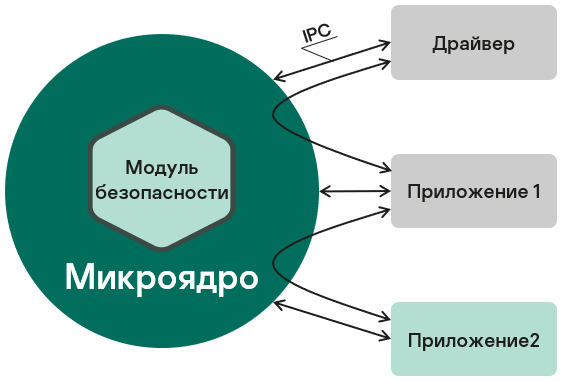
\includegraphics[width=0.75\textwidth]{img/kos_ce_mils_flask.png}
		\caption{Взаимодействие процессов между собой и с ядром в KasperskyOS}
		\label{fig:KasperskyOS}
	\end{figure} 
	
	\item \textbf{Поддержка POSIX}. \newline
	Поддержка около 98\% POSIX API \cite{KasperskyOS_techdata}.
	
	\item \textbf{Портирование}. \newline
	KasperskyOS работает на платформах Intel x86/x86-64, ARMv5, ARMv7, ARMv8 и MIPS32. Поддержка других аппаратных платформ с MMU может быть организована по запросу.
	
	\item \textbf{Поддержка аппаратной виртуализации}. \newline
	KasperskyOS может использоваться как основа для безопасного гипервизора\footnote{Гипервизор --- программа или аппаратная схема, обеспечивающая одновременную работу нескольких ОС на одном компьютере.} с поддержкой технологий Intel VT-x и VT-d.
	
	\item \textbf{Сокращение поверхности потенциальной атаки}. \newline
	Разделение приложений на домены безопасности и полный контроль междоменных взаимодействий позволяет безопасно использовать потенциально уязвимые и/или недоверенные приложения.
\end{enumerate}



\subsubsection{TinyOS}

TinyOS \cite{TinyOS_main} --- это операционная система с открытым исходным кодом под лицензией BSD, предназначенная для беспроводных устройств с низким энергопотреблением, таких как те, которые используются в сенсорных сетях (Wireless sensor networks), повсеместных вычислениях (ubiquitous computing), персональных сетях, умных зданиях и счетчиках.

% A worldwide community from academia and industry use, develop, and support the operating system as well as its associated tools, averaging 35,000 downloads a year.

Архитектура TinyOS включает две главные функциональные составляющие: планировщик задач и компонент \cite{TinyOS_BMSTU}. Понятие <<компонент>> в TinyOS несколько отличается от общепринятого. Так, интерфейс компонента TinyOS состоит из двух частей: верхней (upper), предоставляемой этим компонентом как провайдером, и нижней (lower), требуемой для его функционирования. Обе части содержат описания команд и событий.

TinyOS имеет компонентную модель программирования \cite{TinyOS_book}, кодифицированную языком NesC, являющегося диалектом языка C. TinyOS не является ОС в традиционном понимании. Это программная платформа для встраиваемых систем и набор компонентов, которые позволяют встраивать ОС, специфичную для каждого приложения. Типичное приложение имеет размер около 15K, из которых базовая ОС занимает около 400 байт. Размер самого большого приложения, системы запросов, подобной базе данных, составляет около 64 Кбайт.

Приложение на TinyOS представляет собой граф компонентов, каждый из которых является независимым объектом, который предоставляет один или несколько интерфейсов. Компоненты имеют три вычислительные абстракции: команды, события и задачи. Команды и события --- это механизмы для межкомпонентного взаимодействия, в то время как задачи используются для выражения внутрикомпонентного параллелизма.





\subsubsection{Ubuntu Core}

Ubuntu Core \cite{Ubuntu_Core_doc} --- это версия операционной системы Ubuntu \cite{Ubuntu_Desktop}, разработанная и спроектированная для IoT и встраиваемых систем. Данная операционная система обновляет себя и свои приложения автоматически. Пакеты Snap используются исключительно для создания замкнутой и основанной на транзакциях системы.

Ubuntu Core можно запускать как виртуальную машину или на следующих платформах:

\begin{itemize}[label*=---]
	\item Raspberry Pi 2 and 3;
	\item Compute Module 3;
	\item Qualcomm DragonBoard 410c;
	\item Intel NUC;
	\item Intel Joule;
	\item Samsung Artik;
	\item KVM;
	\item Amazon Web Services (AWS);
	\item Microsoft Azure;
	\item Google Cloud Platform.
\end{itemize}

Ubuntu Core \cite{Ubuntu_Core_def} --- это транзакционная версия ОС Ubuntu Linux, созданная специально для устройств интернета вещей и развертывания больших контейнеров. Эта ОС использует то же ядро, библиотеки и системное программное обеспечение, что и стандартная Ubuntu, но в гораздо меньших масштабах.

Транзакционные операционные системы делят работу на полные, неделимые операции. Ubuntu Core работает за счет использования моментальных пакетов. Snaps --- это zip-файлы, которые содержат контейнерное приложение и его зависимости, а также инструкции по безопасному запуску и взаимодействию с другим программным обеспечением. Snap запускаются на любом Linux (для ПК, сервера или облачного устройства), изолированном от базовой ОС для безопасной установки приложения.

Snap доступны только для чтения и являются неизменяемыми, что предотвращает любые изменения при установке в системе. Наряду с приложением и его зависимостями снимки содержат два отдельных пространства для хранения с возможностью записи, одно из которых является версионным и сохраняет копии любых обновлений данных, а другое хранит большие объемы статических данных, не требующих повторного дублирования.



\subsubsection{Raspbian}

Raspbian \cite{Raspbian_overview} --- это операционная система с открытым исходным кодом, основанная на Debian и оптимизированная для аппаратной платформы Raspberry Pi.

Raspbian --- это неофициальный перенос Debian Wheezy armhf \cite{Debian_Wheezy} с настройками компиляции, скорректированными для получения оптимизированного кода <<hard float>>, который будет работать на Raspberry Pi. Это обеспечивает значительно более высокую производительность для приложений, интенсивно использующих арифметические операции с плавающей запятой. Все остальные приложения также получают определенный прирост производительности за счет использования расширенных инструкций процессора ARMv6 в Raspberry Pi.

Ниже представлены ключевые особенности Raspbian.
\begin{enumerate}[label*=\arabic*.]
	\item \textbf{Пользовательский интерфейс}. \newline
	Raspbian имеет среду рабочего стола PIXEL, основанную на LXDE \cite{LXDE}, которая похожа на многие распространенные рабочие столы, такие как macOS и Microsoft Windows. Рабочий стол имеет фоновое изображение. Строка меню расположена вверху и содержит меню приложений и ярлыки для веб-браузера (Chromium), файлового менеджера и терминала. На другом конце строки меню отображаются меню Bluetooth , меню Wi-Fi, регулятор громкости и часы. Рабочий стол также можно изменить по сравнению с его внешним видом по умолчанию, например, изменить положение строки меню \cite{Raspbian_customize}.
	
	\item \textbf{Управление пакетами}. \newline
	Пакеты можно устанавливать через пакетный менеджер APT \cite{APT}, используемый во всех операционных системах, основанных на Debian. Взаимодействие с APT возможно как через консольный, так и через графический интерфейс.
	
	\item \textbf{Компоненты}.
	\subitem PCManFM — это файловый браузер, обеспечивающий быстрый доступ ко всем областям компьютера.
	\subitem Raspberry Pi OS распространяется с веб-браузером Chromium. Встроенный браузер поставляется с предустановленными uBlock Origin и h264ify.
	\subitem Raspberry Pi OS поставляется с IDE, такими как Thonny Python IDE, Mu Editor и Greenfoot. Он также поставляется с образовательным программным обеспечением, таким как Scratch и Bookshelf.
	
\end{enumerate}

\pagebreak